\section{Backpropagation}

\subsection{Notation}

Um in einem mehrschichtigen Netz effizient die Kostenfunktion zu minimieren wird in vielen Fällen der \emph{Backpropagation}-Algorithmus verwendet. Dieser wurde bereits in den Siebzigerjahren definiert, erlangt jedoch erst im Jahr 1986 mit dem Paper \emph{Learning representations by back-propagating errors} von Rumelhart, Hinton und Williams Bekanntheit. 

Im vorherigen Teil habe ich bereits beschrieben was man unter dem Gradientenabstieg versteht und wie dieser auch bei mehrdimensionalen Funktionen (wie zum Beispiel der hierbei betrachteten Kostenfunktion) verwendet werden kann. Es wurde jedoch noch nicht vorgestellt, wie man auf ein mehrschichtiges Netz bezogen, diesen Gradienten überhaupt berechnen kann. 

Gemeinhin wird die Notation wie sie in Abbilung \ref{fig:weight_not} zu sehen ist, für ein Gewicht verwendet. In Abbildung \ref{fig:biasAct_not} steht das $b^l_j$ für den Schwellwert (\emph{Bias}) am Neuron mit dem Index \emph{j} im Layer mit dem Index \emph{l}. Selbes gilt für die Aktivierung welche mit einem \emph{a} gekennzeichnet wird. Mit den gegebenen Notationen können wir folgende Gleichung für die Aktivierung eines Neurons aufstellen (siehe Gleichung \ref{eq:act}). 

\begin{figure}[!htb]
	\centering
	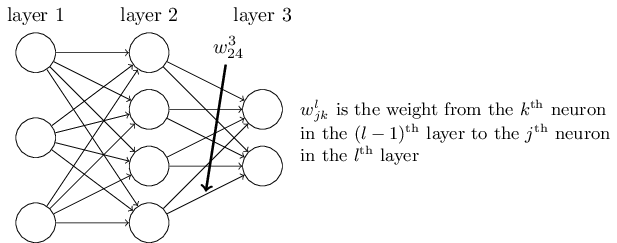
\includegraphics[width=\linewidth]{img/weight_notation}
	\mycaption{Notation}{dlnielsen}
	\label{fig:weight_not}
\end{figure}

\begin{figure}[!htb]
	\centering
	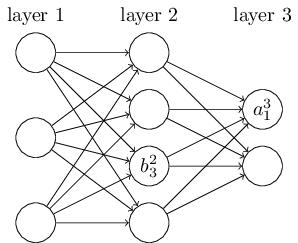
\includegraphics[width=.4\linewidth]{img/biasAct_notation}
	\mycaption{Notation}{dlnielsen}
	\label{fig:biasAct_not}
\end{figure}

\begin{equation} \label{eq:act}
a^{l}_j = \sigma\left( \sum_k w^{l}_{jk} a^{l-1}_k + b^l_j \right),
\end{equation}

Diese Formel sollte bereits aus den vorherigen Kapiteln bekannt sein. Es wird hierbei lediglich eine Vektormultiplikation der beiden eingehenden Gewichtsvektors und Addition mit den Aktivierungsvektoren durchgeführt. Die generierte Ausgabe wird mit dem Schwellwert verrechnet und in eine Aktivierungsfunktion (wie sum Beispiel der Sigmoid-Funktion) gesteckt.

Um später einfacher mit all diesen Werten zu rechnen wird versucht die gegebenen Werte in eine Matrix- beziehungsweise Vektor-Darstellungsform zu bringen. Da Neuron mehrere ausgehende \myquote{Pfade} besitzen wird hierbei eine Matrix geformt. Das bisher beschriebene Gewicht $w^l_{jk}$ befindet sich hierbei in der Zeile mit dem Index \emph{j} und Spaltenindex \emph{k}. Da sich sowohl der Schwellwert als auch die Aktivierung lediglich auf ein einzelnes Neuron beziehen muss hierfür lediglich ein eindimensionaler Vektor pro Layer \emph{l} generiert werden. Die einzelnen Komponenten werden hierbei über den Index \emph{j} angesteuert. Die Notation für den Aktivierungsvektor der Schicht \emph{l} sieht dann derartig aus: $a^l_j$. Ähnliches gilt fur die Schwellwerte: $b^l_j$. 

Um mit diesen Vektoren arbeiten zu können muss man die abschließende Aktivierungsfunktion $\sigma$ vektorisieren 
\footnote{Klarer Verweis auf Nielsen Buch, Kapitel über Backpropagation im Detail \cite{dlnielsen}}. 
Dabei muss man die Funktion lediglich derartig umschreiben, dass diese auf die einzelnen Komponenten angewendet wird und nicht auf einen einzelnen Wert. Beispielsweise würde die Funktion $f(x) = x^2$ vektorisiert folgendermaßen aussehen: 

\begin{equation}
  f\left(\left[ \begin{array}{c} 2 \\ 3 \end{array} \right] \right)
  = \left[ \begin{array}{c} f(2) \\ f(3) \end{array} \right]
  = \left[ \begin{array}{c} 4 \\ 9 \end{array} \right],
\end{equation}

Mit diesen Zusammenfassungen kann nun die Gleichung \ref{eq:act} folgendermaßen umgeschrieben werden: 

\begin{equation}
  a^{l} = \sigma(w^l a^{l-1}+b^l).
\end{equation}

Diese Umschreibung abstrahiert das Denken über die lokalen Neuronen auf ein höheres Level sodass es einfacher ist das Gesamtbild zu betrachten. Um noch mehr Klarheit zu schaffen wird oftmals die Aktivierung einer Schicht \emph{l} aus der Funktion herausgezogen und mit dem Buchstaben \emph{z} versehen. $z^l$ kann nun in die Aktivierungsfunktion $\sigma$ eingesetzt werden. Im folgenden habe ich noch einmal alle bisherigen Erkenntnisse zusammengefasst: 

\begin{mytheo}{Backpropagation - Notation}{theoexample}

Bisherige Schreibweise:
\begin{equation}
  a^{l}_j = \sigma\left( \sum_k w^{l}_{jk} a^{l-1}_k + b^l_j \right) \nonumber
\end{equation}

Zusammengefasste Form:
\begin{equation}
a^l = \sigma(z^l)
\end{equation}

Gewichtete Eingabe:
\begin{equation}
  z^l \equiv w^l a^{l-1}+b^l
\end{equation}

\end{mytheo}

\subsection{Fundamentale Gleichungen}

Ziel des Backpropagation Algorithmus ist es 